\section{Herleitung der Modelldynamik}
\label{sec:herleitung_der_modelldynamik}

Die den Pendelmagneten beeinflussenden Kräfte können in zwei Kategorien unterteilt werden:

\paragraph{Äußere Einwirkungen} Am offensichtlichsten ist die Gesamtheit der äußeren Einwirkungen $\vec{F}_{ges}$, also alle Kräfte, die nicht in Zusammenhang mit der Kreisbewegung des Pendels stehen. Diese bestehen aus der Erdanziehungskraft $\vec{F}_{g}$, der zwischen dem Pendelmagneten und den festen Ablenkungsmagneten wirkenden Coulombkraft $\vec{F}_{c}$ und dem Strömungswiderstand $\vec{F}_{fr}$. Daraus ergibt sich folgende Formel:

\begin{align} \label{f_ges}
    \vec{F}_{ges} &= \vec{F}_{g} + \vec{F}_{fr} + \vec{F}_{c}
\end{align}

Diese Kraft muss dann mithilfe einer in Teilabschnitt \ref{ssec:die_kräftezerlegung} beschriebenen Kräftezerlegung aufgespalten werden - in ihren tangential zur Pendelbewegung wirkenden Teil $\vec{F}_{tan}$ und den normal zur Selbigen wirkenden Teil $\vec{F}_{norm}$. $\vec{F}_{ges}$ ist somit auch die Summe dieser beiden Teilkräfte.

\begin{align} \label{f_ges_kräftezerlegung}
    \vec{F}_{ges} &= \vec{F}_{tan} + \vec{F}_{norm}
\end{align}

\paragraph{Zugkraft der Verbindungsstange} Die restlichen Kräfte sind unter der Zugkraft der Verbindungsstange $\vec{F}_{zug}$ vereint. Sie halten den Pendelmagneten in seiner Kreisbahn. Dazu zählen die Zentripetalkraft $\vec{F}_{zp}$, sowie die der Normalkraft $\vec{F}_{norm}$ entgegenwirkenden Kraft $\vec{F}_{geg}$. Diese ist dafür verantwortlich, dass der Pendelmagnet von den magnetischen Anziehungskräften oder der Gewichtskraft nicht nach unten gezogen werden kann, was eine Verlängerung der imaginären Verbindungsstange zur Folge hätte. Die Formel für die Zugkraft der Verbindungsstange ergibt sich aus folgender Herleitung:

\begin{align*}
    \vec{F}_{geg} &= - \vec{F}_{norm}\\
    \vec{F}_{zug} &= \vec{F}_{zp} + \vec{F}_{geg}
\end{align*}
\begin{align} \label{f_zug}
    \vec{F}_{zug} &= \vec{F}_{zp} - \vec{F}_{norm}
\end{align}

\subsection{Die Erdanziehungskraft}
\label{ssec:die_erdanziehungskraft}

Für die Berechnung des Betrags der Erdanziehungskraft gilt folgende Formel, wobei $m$ die Masse der Pendelkugel ist und $g$ die Erdbeschleunigung darstellt.

\begin{align*}
    F_{g} &= m \cdot g
\end{align*}

Die Richtung der Erdbeschleunigung entspricht der Richtung zum Erdmittelpunkt vom betrachteten Objekt aus. In Anbetracht der Größenverhältnisse zwischen Modell und Erde kann die Richtung von $\vec{F}_{g}$ aber als senkrecht nach unten zeigend angenommen werden. Es ergibt sich somit folgende Formel für die Berechnung der Erdanziehungskraft im Modell.

\begin{align} \label{f_g}
    \vec{F}_{g} &= m \cdot g \cdot \cvec{0}{0}{-1}
\end{align}

\subsection{Der Strömungswiderstand}
\label{ssec:der_strömungswiderstand}

Der Betrag des Strömungswiderstands lässt sich mit dieser Formel berechnen.

\begin{align*}
    F_{fr} &= \frac{1}{2} \cdot A \cdot c_{w} \cdot \rho \cdot v^2
\end{align*}

Dabei ist $\rho$ die Dichte des Mediums, $v$ die relative Geschwindigkeit des Objekts zum Medium und $A$ dessen maximale Querschnittsfläche in der Senkrechten zu seiner relativen Bewegungsrichtung. Der sogenannte $c_{w}$-Wert oder Strömungswiderstandskoeffizient bezieht sich auf das Objekt, und beschreibt dessen Aerodynamik. Zu beachten ist, wenn es um die Betrachtung der Reibung geht, dass die Verbindungsstange, die in der Realität notwendig ist, um die Kugel in ihrer Kreisbahn zu halten, im Modell nur eine unsichtbare Kraft ist, beziehungsweise als unendlich dünne Stange implementiert ist. Daraus ergibt sich, dass jegliche Reibung, die zwischen Stange und Medium oder an einer Verankerung der Stange am Koordinatenursprung entsteht vernachlässigt wird. Sei $r$ der Radius der Pendelkugel, werden der Betrag des Strömungswiderstands und die dabei relevanten Komponenten folgendermaßen berechnet.

\begin{align*}
    A &= r^2 \cdot \pi \\
    F_{fr} &= \cfrac{1}{2} \cdot r^2 \pi \cdot c_{w} \cdot \rho \cdot v^2
\end{align*}

Nachdem der Betrag des Strömungswiderstands nun berechnet ist, gilt es jetzt den vollständigen Vektor zu bilden. Da die Kraft, die den Strömungswiderstand darstellt, immer entgegengesetzt der Bewegungsrichtung wirkt, ist es zunächst notwendig den Einheitsvektor der Pendelgeschwindigkeit $\vec{v}$ zu ermitteln, was durch das Dividieren derselben durch ihren Betrag erreicht werden kann.

\begin{align*}
    \vec{v}_{0} &= \cfrac{\vec{v}}{v}
\end{align*}

Nun kann man den Betrag des Strömungswiderstands mit dem negativen Einheitsvektor der Relativgeschwindigkeit multiplizieren und erhält dann die Formel für den Kraftvektor $\vec{F}_{fr}$.

\begin{align*}
    \vec{F}_{fr} &= \cfrac{1}{2} \cdot r^2 \pi \cdot c_{w} \cdot \rho \cdot v^2 \cdot \left(- \vec{v}_{0} \right)
\end{align*}

\begin{align} \label{f_fr}
    \vec{F}_{fr} &= \cfrac{1}{2} \cdot r^2 \pi \cdot c_{w} \cdot \rho \cdot v \cdot (-\vec{v})
\end{align}


\subsection{Die Coulombkräfte}
\label{ssec:die_coulombkräfte}

Wie bereits angemerkt, werden die Magnete im Modell wie elektrisch geladene Kugeln behandelt. Das bietet den Vorteil, dass die Berechnung der dadurch entstehenden Kräfte deutlich erleichtert wird. Es gilt nämlich ohne Einschränkung das Superpositionsprinzip, das heißt, wenn zwei Fixmagnete am Boden eine Wechselwirkung mit dem Pendelmagneten eingehen, dürfen die Vektoren beider Kräfte vektoriell addiert werden. Des weiteren kann die Berechnung des Betrags der Coulombkraft zwischen zwei kugelförmigen Ladungsträgern $L1$ und $L2$ über folgende Formel vollzogen werden, wenn $Q_{L1}$ und $Q_{L2}$ deren Ladungen sind.

\begin{align*}
    F_{c} &= \bigg\vert\  \cfrac{1}{4\pi \cdot \epsilon_{0} \cdot \epsilon_{r}} \cdot \cfrac{Q_{L1} \cdot Q_{L2}}{\overline{L1L2}^2}\  \bigg\vert
\end{align*}

Da sich gleiche Ladungen immer abstoßen und ungleiche sich anziehen, ergäbe sich, würden keine Betragsstriche verwendet, für den Betrag der Ladung bei einer anziehenden Wirkung ein negativer Wert. Diese Tatsache klingt zwar in sich widersprüchlich, heißt aber nur, dass sich im Betrag schon eine Richtung befindet. Um nun einen korrekt gerichteten Vektor zu erhalten, darf für die Berechnung des Vektors $\vec{F}_{cL1_{L2}}$ nicht der Betrag mit dem Einheitsvektor $\vec{L1L2}_{0}$ multipliziert werden. Bei einer Anziehung würde sonst der negative Betragswert mit der korrekten Vektorrichtung multipliziert, was in einem Vektor mit genau entgegengesetzter Richtung resultieren würde. Stattdessen muss der Einheitsvektor $\vec{L2L1}_{0}$ verwendet werden. Es ergibt sich somit zunächst folgende Formel.

\begin{align*}
    \vec{F}_{cL1_{L2}} &= \cfrac{1}{4\pi \cdot \epsilon_{0} \cdot \epsilon_{r}} \cdot \cfrac{Q_{L1} \cdot Q_{L2}}{\overline{L1L2}^2} \cdot \vec{L2L1}_{0} \\
                  &= \cfrac{Q_{L1} \cdot Q_{L2}}{4 \pi \cdot \epsilon_{0} \cdot \epsilon_{r}} \cdot \cfrac{1}{\overline{L2L1}^2} \cdot \cfrac{\vec{L2L1}}{\overline{L2L1}} \\
                  &= \cfrac{Q_{L1} \cdot Q_{L2}}{4 \pi \cdot \epsilon_{0} \cdot \epsilon_{r}} \cdot \cfrac{\vec{L2L1}}{\overline{L2L1}^{3}}
\end{align*}

Betrachtet man nun die Kraft $\vec{F}_{cP_A}$, die der Pendelmagnet $P$ durch den Ablenkungsmagneten $A$ erfährt, und die Kraft $\vec{F}_{cP_B}$, mit der $B$ den Pendelmagneten ablenkt, so ergeben sich folgende Formeln, aus denen schließlich die gesamte auf $P$ einwirkende Coulombkraft $\vec{F}_{c}$ errechnet werden kann.

\begin{align*}
    \vec{F}_{cP_A} &= \cfrac{Q_{P} \cdot Q_{A}}{4 \pi \cdot \epsilon_{0} \cdot \epsilon_{r}} \cdot \cfrac{\vec{AP}}{\overline{AP}^{3}} \\
    \vec{F}_{cP_B} &= \cfrac{Q_{P} \cdot Q_{B}}{4 \pi \cdot \epsilon_{0} \cdot \epsilon_{r}} \cdot \cfrac{\vec{BP}}{\overline{BP}^{3}} \\
    \vec{F}_{c} &= \vec{F}_{cP_A} + \vec{F}_{cP_B} \\
                 &= \cfrac{Q_{P} \cdot Q_{A}}{4 \pi \cdot \epsilon_{0} \cdot \epsilon_{r}} \cdot \cfrac{\vec{AP}}{\overline{AP}^{3}} + \cfrac{Q_{P} \cdot Q_{B}}{4 \pi \cdot \epsilon_{0} \cdot \epsilon_{r}} \cdot \cfrac{\vec{BP}}{\overline{BP}^{3}}
\end{align*}
\begin{align} \label{f_c}
    \vec{F}_{c} &= \cfrac{Q_{P}}{4 \pi \cdot \epsilon_{0} \cdot \epsilon_{r}} \cdot \left(\cfrac{Q_{A} \cdot \vec{AP}}{\overline{AP}^{3}} + \cfrac{Q_{B} \cdot \vec{BP}}{\overline{BP}^{3}}\right)
\end{align}

\subsection{Die Zentripetalkraft}
\label{ssec:die_zentripetalkraft}

Den letzten Einflussfaktor der resultierenden Kraft stellt die Zentripetalkraft dar. Ist $m$ die Masse des Objekts, $v$ der Betrag seiner Geschwindigkeit und $r$ der Radius der vom Objekt durchlaufenen Kreisbahn, so gilt diese Formel für den Betrag der Zentripetalkraft.

\begin{align*}
    F_{zp} &= m \cdot \cfrac{v^2}{r} \\
           &= m \cdot \cfrac{v^2}{\overline{P0}}
\end{align*}

Um letztendlich den Vektor der Zentripetalkraft zu erhalten, wird ähnlich wie bei den zuvor behandelten Teilkräften der errechnete Betrag mit dem Einheitsvektor, der die Richtung enthält, multipliziert. Hierfür kann der Einheitsvektor $\vec{P0}_{0}$ verwendet werden, da er die imaginäre Stange darstellt, von der die Zentripetalkraft zum Kreismittelpunkt hin aufgebracht wird.

\begin{align*}
    \vec{F}_{zp} &= m \cdot \cfrac{v^2}{\overline{P0}} \cdot \vec{P0}_{0} \\
                 &= m \cdot \cfrac{v^2}{\overline{P0}} \cdot \cfrac{\vec{P0}}{\overline{P0}}
\end{align*}
\begin{align} \label{f_zp}
    \vec{F}_{zp} &= m v^2 \cdot \cfrac{\vec{P0}}{\overline{P0}^2}
\end{align}

\subsection{Die Kräftezerlegung}
\label{ssec:die_kräftezerlegung}

Um ermitteln zu können, welche Teilkraft $\vec{F}_{geg}$ die Verbindungsstange aufbringen muss, muss der normal zur Pendelbahn gerichtete Teil $\vec{F}_{norm}$ von $\vec{F}_{ges}$ ermittelt werden. Dieser ist genau der Teil, der von der Stange absorbiert werden muss, um eine Entfernung des Pendelmagneten vom Ankerpunkt zu verhindern. Der andere Teil von $\vec{F}_{ges}$ hingegen, $\vec{F}_{tan}$ ist tangential zur Pendelbahn ausgerichtet und stellt somit alle Kräfte dar, die die Auslenkung des Pendels beeinflussen. Abbildung \ref{fig:skizze_der_kräftezerlegung} zeigt alle dabei relevanten Kräfte im Modell.

\begin{figure}
    \includegraphics{kraeftezerlegung}
    \caption{Skizze der Kräftezerlegung}
    \label{fig:skizze_der_kräftezerlegung}
\end{figure}

\paragraph{Normalkraft} Zur Bestimmung von $\vec{F}_{norm}$ muss eine orthogonale Zerlegung am Vektor $\vec{F}_{ges}$ durchgeführt werden. Dabei gilt, wie in \cite{meyberg2013hoehere} genauer erklärt wird, dass die Komponente $\vec{a}_{b}$ eines Vektors $\vec{a}$ mit folgender Formel bestimmt werden kann, wenn $\vec{b}$ die Richtung von $\vec{a}_{b}$ vorgibt.

\begin{align*}
    \vec{a}_{b} &= \cfrac{\vec{a} \circ \vec{b}}{b^2} \cdot \vec{b}
\end{align*}

Wendet man dies auf die Kräftezerlegung an $\vec{F}_{ges}$ an, so ergibt sich diese Formel für die Kraft $\vec{F}_{norm}$, da sie die selbe Richtung wie die Verbindungsstange, also der Vektor $\vec{0P}$, hat.

\begin{align} \label{f_norm}
    \vec{F}_{norm} &= \cfrac{\vec{F}_{ges} \circ \vec{0P}}{\overline{0P}^2} \cdot \vec{0P}
\end{align}

\paragraph{Tangentialkraft} Wie am Anfang des Abschnitts \ref{sec:herleitung_der_modelldynamik} bereits erläutert wurde, ist die Tangentialkraft $\vec{F}_{tan}$ der rechtwinklig zur Normalkraft ausgerichtete Teil der Kraft $\vec{F}_{ges}$. Sie ist also, wie der Name impliziert, tangential zur Bahn des Pendels ausgerichtet und stellt somit den Antrieb für jegliche Richtungsänderung auf der Kreisbahn des Pendelmagneten dar. Da $\vec{F}_{ges}$ und $\vec{F}_{norm}$ bereits bekannt sind, kann $\vec{F}_{tan}$ durch eine Subtraktion errechnet werden.

\begin{align} \label{f_tan}
    \vec{F}_{tan} &= \vec{F}_{ges} - \vec{F}_{norm}
\end{align}

\paragraph{Resultierende Kraft} Zur Ermittlung der resultierenden Kraft $\vec{F}_{res}$ müssen sämtliche Kräfte, also die Gesamtheit der äußeren Einwirkungen $\vec{F}_{ges}$ und die Zugkraft der Verbindungsstange $\vec{F}_{zug}$, addiert werden.

\begin{align*}
    \vec{F}_{res} &= \vec{F}_{ges} + \vec{F}_{zug}
\end{align*}

Setzt man hier zunächst die Formeln \eqref{f_ges_kräftezerlegung} und \eqref{f_zug} ein und ersetzt anschließend $\vec{F}_{tan}$ durch die zuvor dafür aufgestellte Formel \eqref{f_tan}, so ergibt sich folgende Umformung:

\begin{align*}
    \vec{F}_{res} &= \vec{F}_{tan} + \vec{F}_{norm} + \vec{F}_{zp} - \vec{F}_{norm} \\
                  &= \vec{F}_{tan} + \vec{F}_{zp} \\
                  &= \vec{F}_{ges} - \vec{F}_{norm} + \vec{F}_{zp}
\end{align*}

Ersetzt man schließlich die Normalkraft durch die Formel \eqref{f_norm}, so sind auch alle abstrakteren Größen eliminiert.

\begin{align} \label{f_res}
    \vec{F}_{res} &= \vec{F}_{ges} - \cfrac{\vec{F}_{ges} \circ \vec{0P}}{\overline{0P}^2} \cdot \vec{0P} + \vec{F}_{zp}
\end{align}

\subsection{Die Differentialgleichungen}
\label{ssec:die_differentialgleichungen}

Um aus der zuvor bestimmten resultierenden Kraft die Änderung von Geschwindigkeit und Position zu ermitteln, sind nur wenige Formeln nötig. Zunächst kann die auf den Pendelmagneten wirkende Beschleunigung gemäß dem 2. Newtonschen Gesetz über diese Formel bestimmt werden:
\begin{align} \label{a}
	\vec{a} &= \cfrac{\vec{F}}{m}
\end{align}
Für die Geschwindigkeitsänderung $\dot{\vec{v}}$ und die Positionsänderung $\dot{\vec{p}}$ gelten zudem diese Formeln:
\begin{align} \label{v}
	\dot{\vec{v}} &= \vec{a}
\end{align}
\begin{align} \label{p}
    \dot{\vec{p}} &= \vec{v}
\end{align}